\documentclass[conference,9pt]{IEEEtran}
\IEEEoverridecommandlockouts
\usepackage{cite}
\usepackage{amsmath,amssymb}
\usepackage{graphicx}
\usepackage{booktabs}
\usepackage{xcolor}
\usepackage{listings}
\usepackage[hidelinks]{hyperref}

\lstset{basicstyle=\ttfamily\scriptsize,columns=fullflexible,frame=single,breaklines=true}
\newcommand{\HW}{\mathrm{HW}}
\newcommand{\Sb}{\mathrm{Sbox}}
\newcommand{\ISb}{\mathrm{InvSbox}}

\begin{document}

\title{Side-Channel Analysis of an AES-128 FPGA Core\\Protected by a Fake-Key Countermeasure}

\author{
\IEEEauthorblockN{Team Name: Synapse}\\[4pt]
\IEEEauthorblockN{Rohan Rajeev Bharadwaj, Pugazhendhi G~S, Aryan Anish}\\[2pt]
\IEEEauthorblockA{\{rohanrb25, pugazhendhi25, aaryan25\}@iitk.ac.in}
}

\maketitle

\noindent\textit{Summary}---We attack 100{,}000 power traces of an AES-128 FPGA design whose final round is redirected to a fake key. CPA with a Hamming distance model recovers the fake round-10 key in 2{,}028 traces. The correcting lookup table is functionally a constant XOR, and the first- and second-order attack models we tried on it do not recover the actual key.

\section{Problem}

We are given 100{,}000 power traces (200 samples each) from an AES-128 FPGA core, together with the ciphertext of every encryption. Plaintexts and keys are withheld.

The core implements a recent class of side-channel countermeasure. Instead of hiding the key, it wires a \emph{fake} key into the final round and uses a small precomputed lookup table (LUT) to cancel it, so the device still outputs correct AES ciphertext under its real key. The intent is that a standard CPA attack converges confidently to a key the device never uses.

Our goals:
\begin{itemize}
\item Recover the round-10 key CPA converges on (the fake key).
\item Report how many traces are needed for full 16-byte recovery.
\item Attempt to recover the actual round-10 key and master key.
\end{itemize}

\section{Attack}

\subsection{Leakage model}
At the final clock edge, register cell $j$ changes from $S_9[j]$ to its new value. ShiftRows moves the byte at cell $j = \mathrm{INV\_SR}[i]$ to ciphertext position $i$. Inverting the final round under a key guess $k$ gives the Hamming distance model
\begin{equation}
h_i[k] = \HW\!\big(\ISb(C[i]\oplus k)\oplus C[\mathrm{INV\_SR}[i]]\big).
\label{eq:hd}
\end{equation}
Here INV\_SR is $[0,5,10,15,4,9,14,3,8,13,2,7,12,1,6,11]$, with byte numbering in column-major order.

\subsection{Procedure}
Let $T\in\mathbb{R}^{N\times200}$ be the traces and $H_i\in\mathbb{R}^{N\times256}$ the predictions (\ref{eq:hd}). After centring and normalising columns, the correlation matrix is
\begin{equation}
\rho_i = \tilde{H}_i^{\top}\tilde{T}\in[-1,1]^{256\times200}.
\end{equation}
For each byte we take $\arg\max_k \max_t |\rho_i[k,t]|$, and the maximising $t$ gives the leaking sample. All 16 bytes from 100{,}000 traces are recovered in about 7\,s on a laptop CPU with NumPy.

\section{Results}

\subsection{Trace shape}
Fig.~\ref{fig:mean} shows the mean of the 100{,}000 traces. Periodic oscillations occupy the first 45 samples, the large negative edge at sample $\sim$49 is the update of the final state register, and the trace is flat after $\sim$55. All 16 key bytes peak on this edge.

\begin{figure}[t]
\centering
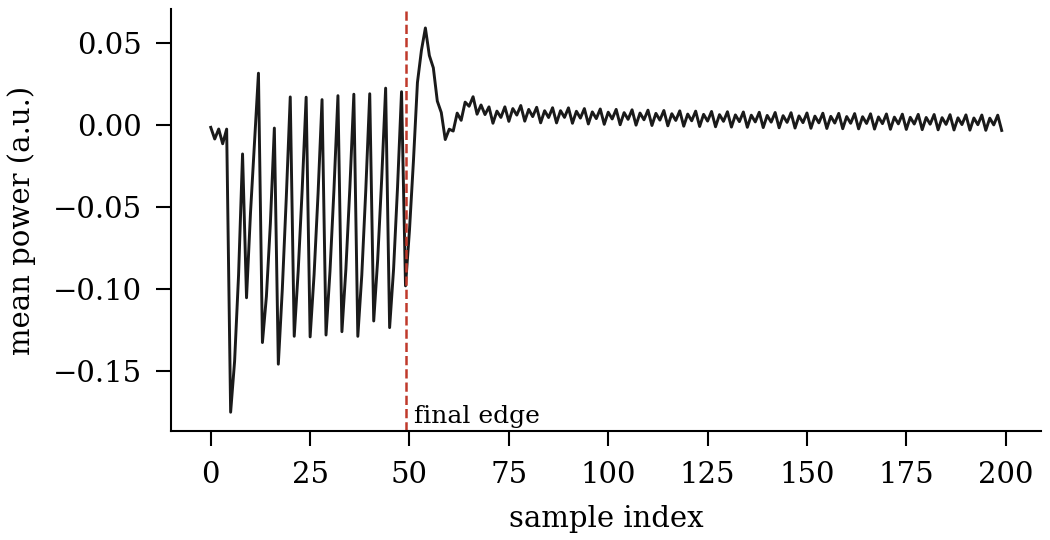
\includegraphics[width=\columnwidth]{figs/mean_trace.png}
\caption{Mean of the 100{,}000 traces. The dashed line marks the sample where the key correlations peak.}
\label{fig:mean}
\end{figure}

\subsection{Recovered fake key}
The attack converges on
\[
\texttt{91dec068e3face4599ce38f420863a30}
\]
for the round-10 key. Every byte peaks at sample 49 or 50, with $|\rho|$ between 0.119 and 0.178 (Fig.~\ref{fig:corr}). The winner beats the runner-up by a factor of 8.3--11.2 for bytes outside the first state row and 3.3--4.1 for bytes 0, 4, 8, 12. The weaker separation for row~0 is expected: for these bytes INV\_SR$[i] = i$, so the model reduces to $\HW(\ISb(C[i]\oplus k)\oplus C[i])$, a Hamming distance between two derived values of the same ciphertext byte, which behaves differently from the other rows. The sign of the correlation is measurement polarity and is not significant; we take absolute values.

\begin{figure*}[t]
\centering
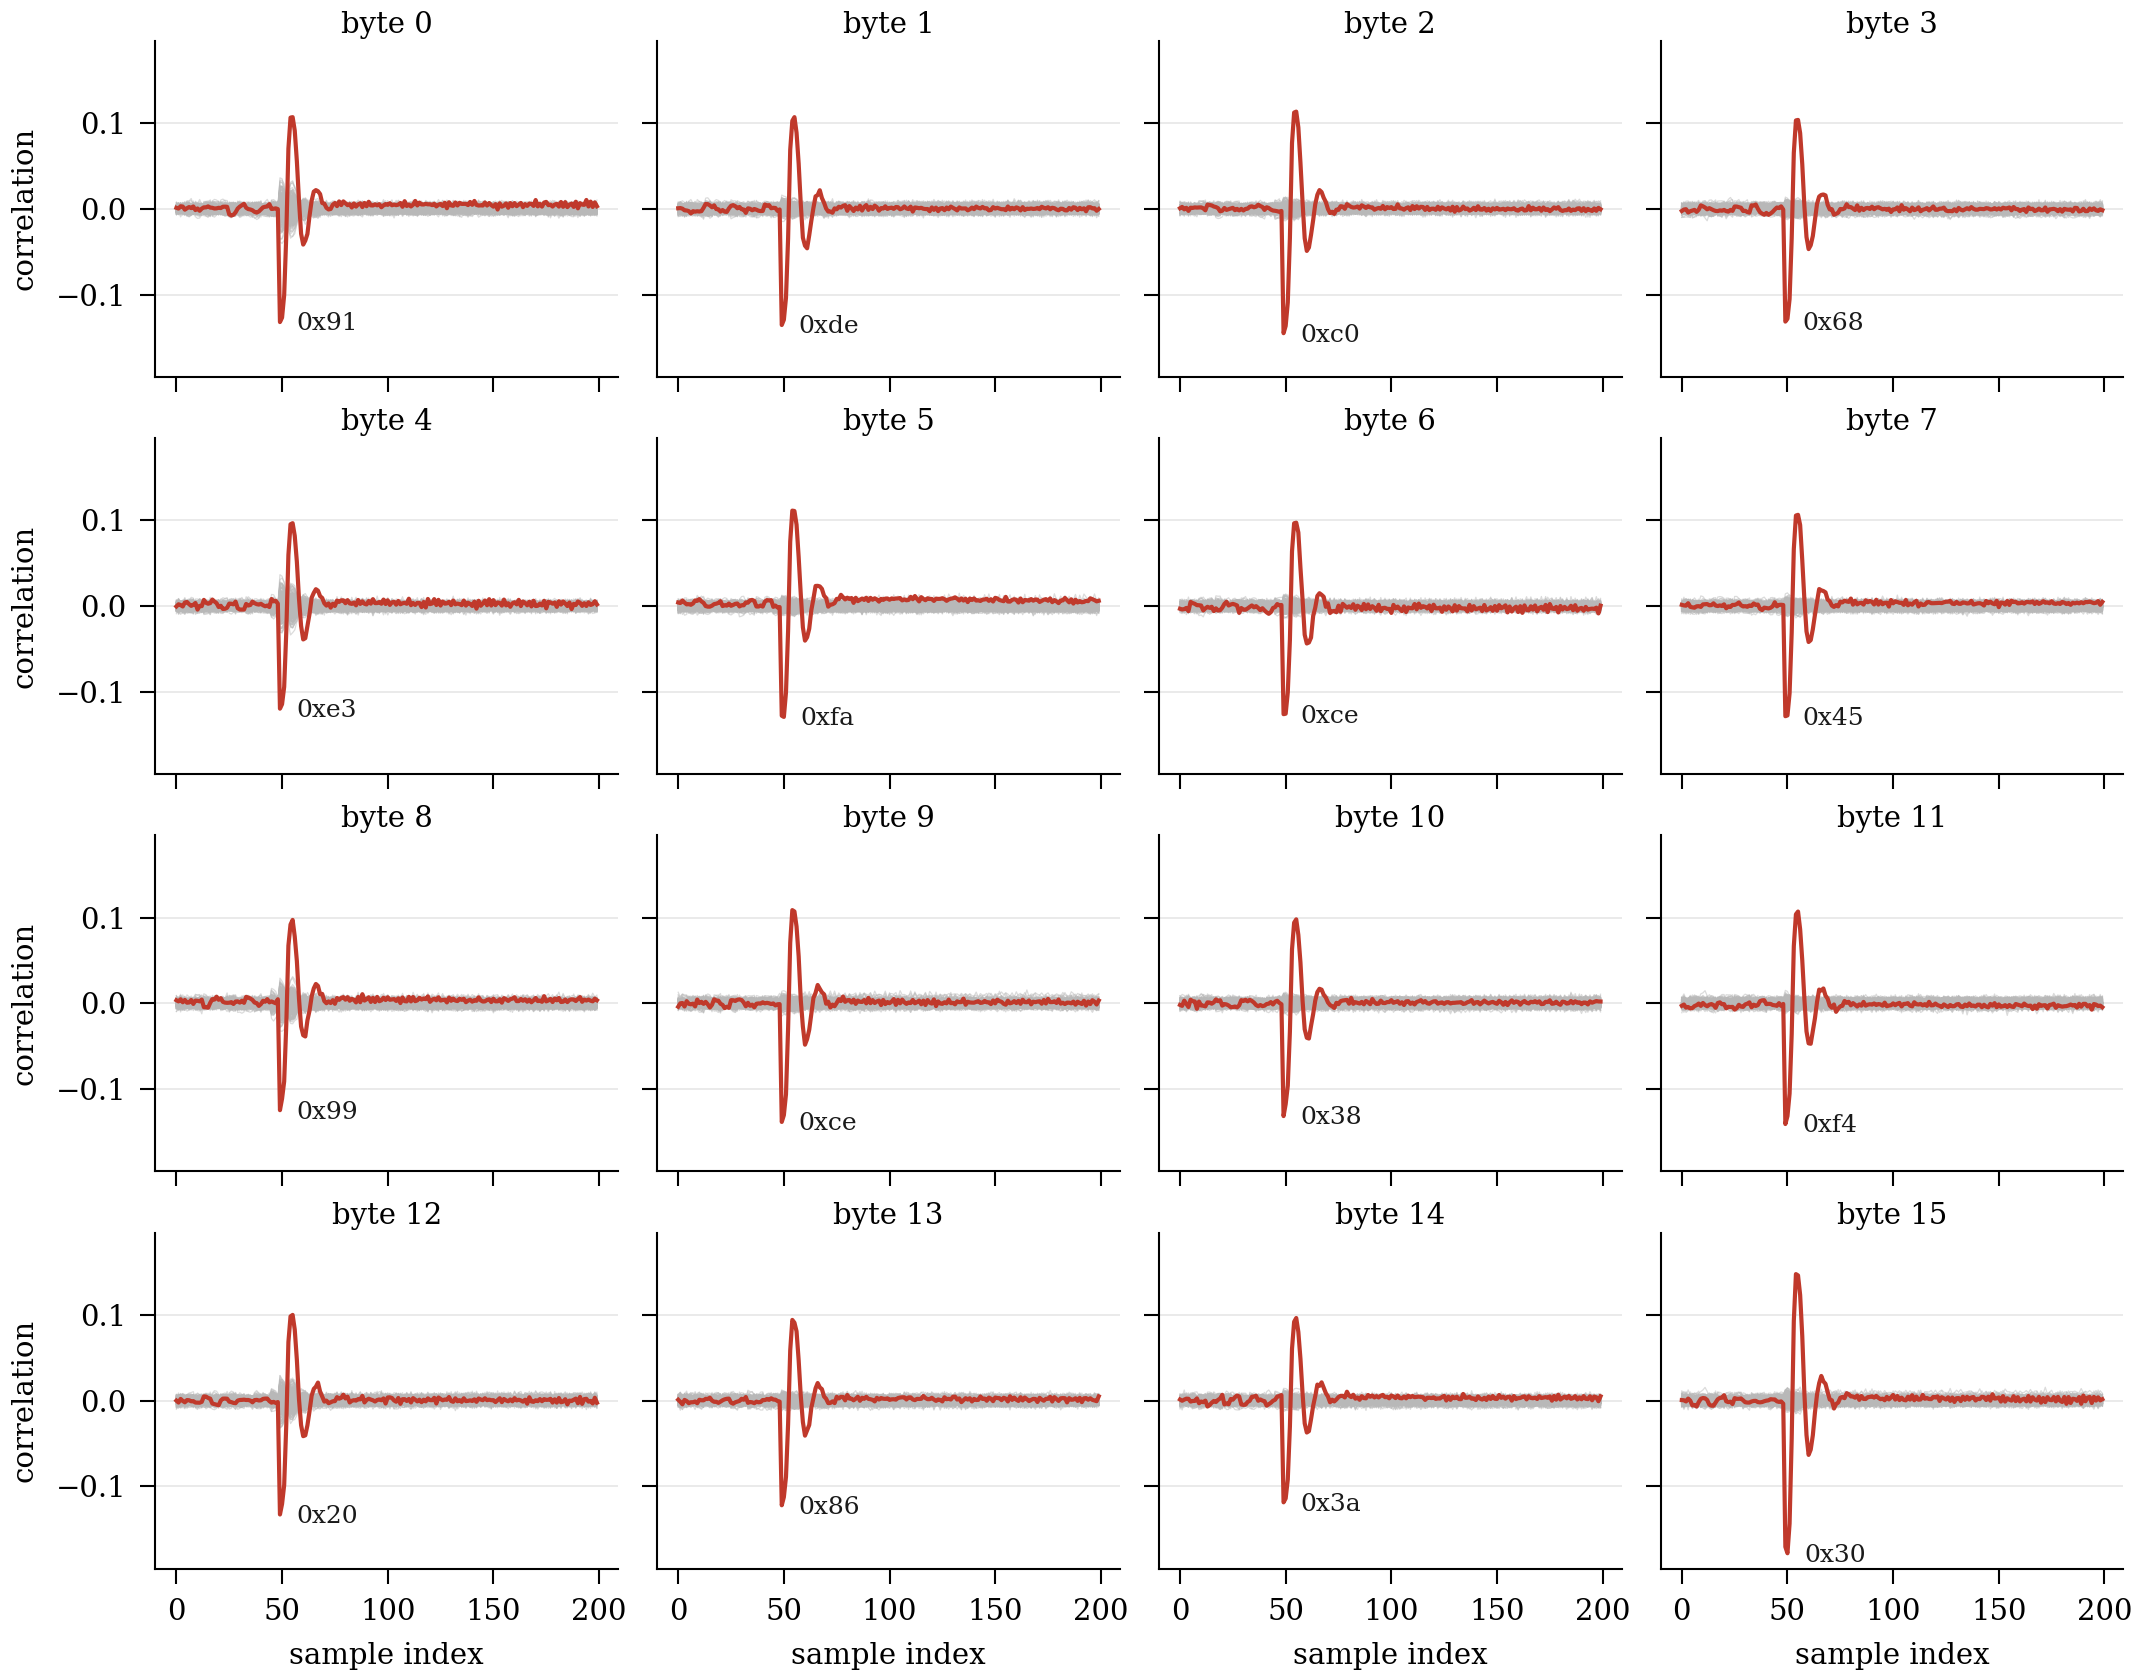
\includegraphics[width=0.92\textwidth]{figs/corr_grid.png}
\caption{Correlation against sample index for all 256 candidates of each key byte. Grey: wrong candidates. Red: winning candidate, labelled with its byte value.}
\label{fig:corr}
\end{figure*}

\subsection{Traces required}
Fig.~\ref{fig:rank} shows the rank of every byte as the number of traces grows. All 16 bytes reach rank 0 and stay there from $N = 2{,}028$ traces onward. Over random subsets the success rate for full 16-byte recovery rises from 5\,\% at 1{,}198 traces to 100\,\% at 3{,}105 (Table~\ref{tab:success}). Fig.~\ref{fig:corrN} compares the correct candidate's peak correlation against the best wrong candidate.

\begin{figure}[t]
\centering
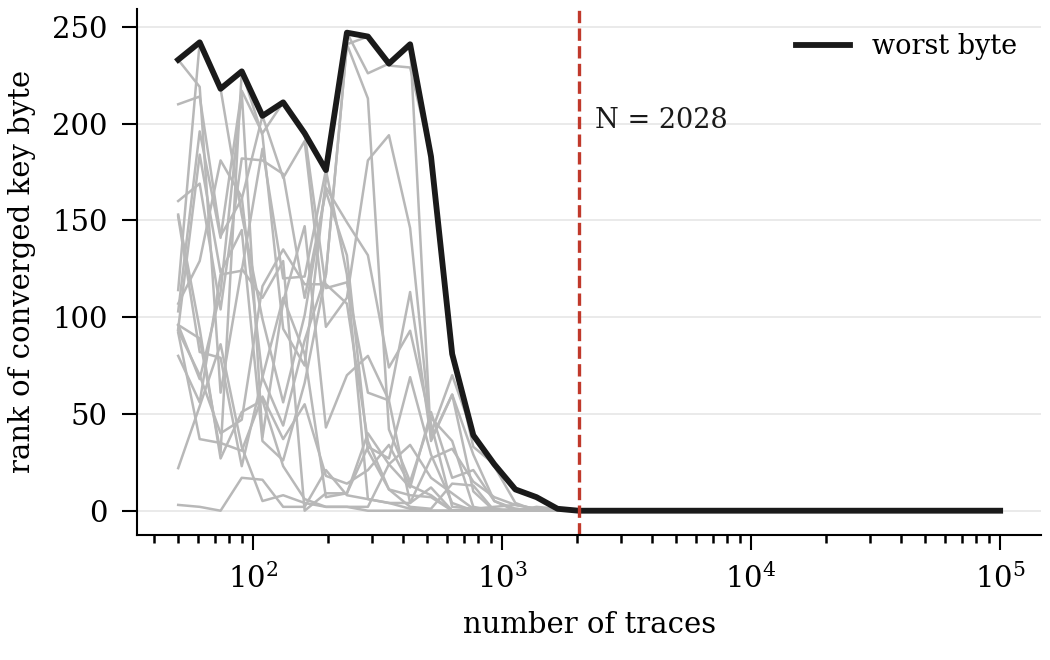
\includegraphics[width=\columnwidth]{figs/rank_vs_n.png}
\caption{Rank of each converged key byte versus number of traces (first $N$ traces). Grey: individual bytes. Black: worst byte.}
\label{fig:rank}
\end{figure}

\begin{figure}[t]
\centering
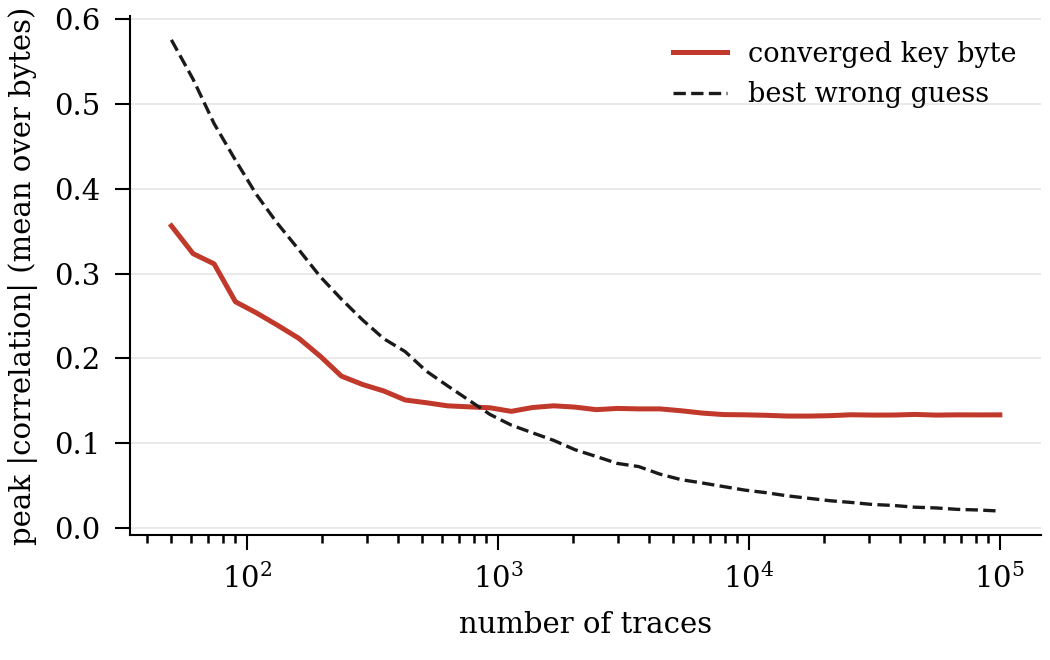
\includegraphics[width=\columnwidth]{figs/corr_vs_n.png}
\caption{Peak $|\rho|$ of the correct candidate against the best wrong candidate, averaged over bytes.}
\label{fig:corrN}
\end{figure}

\begin{table}[t]
\centering
\caption{Success rate of full 16-byte recovery (20 random subsets per $N$).}
\label{tab:success}
\begin{tabular}{@{}lccccccccc@{}}
\toprule
$N$ & 1022 & 1198 & 1404 & 1645 & 2260 & 2649 & 3105 & 3639 & 5000\\
\midrule
Rate & 0.00 & 0.05 & 0.10 & 0.35 & 0.60 & 0.85 & 1.00 & 1.00 & 1.00\\
\bottomrule
\end{tabular}
\end{table}

\section{The Actual Key}

\subsection{The LUT is a constant XOR}
Let $Y = \mathrm{SR}(\Sb(S_9))$. The protected datapath computes $X = Y\oplus F$ with the fake key $F$, and the LUT output must equal the correct ciphertext $C = Y\oplus R$ for every $Y$, where $R = RK_{10}$. Substituting $Y = X\oplus F$:
\begin{equation}
L(X) = X \oplus F \oplus R = X \oplus \Delta, \qquad \Delta = F\oplus R.
\end{equation}
The LUT is therefore functionally a constant XOR, and recovering $R$ is equivalent to recovering $\Delta$. This is a statement about the function the LUT computes. It does not by itself say anything about how much the physical implementation leaks: intermediate values, switching activity, glitches and routing effects can still carry information about $\Delta$ even when the input--output function is a plain XOR.

\subsection{What we tried}
We attacked the LUT with a set of first-order CPA models chosen to cover the natural candidates: $\HW(C[i]\oplus\delta)$, $\HW(\Sb(C[i]\oplus\delta))$, $\HW(\ISb(C[i]\oplus\delta))$ and three Hamming-distance variants against $C[\mathrm{INV\_SR}[i]]$. Each was run over the full 200-sample window and over windows centred on every visible clock edge. The only model that produced a strong peak was the round-register Hamming distance model, and it recovers $\delta = F$ exactly: the fake key again, not the actual key. Every model that targets the LUT directly gave median winner/runner-up ratios of 1.00--1.14, indistinguishable from noise.

We then ran a bivariate centered-product CPA: for each byte, we correlated the model against the product of two centred trace samples over all pairs $(t_1,t_2)$ with $t_1\in[40,60)$ and $t_2\in[42,120)$. This catches leaks in which two samples jointly depend on $\delta$. Median ratios were 1.00 for $\HW(C[i]\oplus\delta)$ and 1.05 for $\HW(\ISb(C[i]\oplus\delta))$, with no consistent peak sample across bytes.

The constant-XOR structure predicts this: any first-order statistic of the LUT input $X = C\oplus\Delta$ is a deterministic function of the observed ciphertext and $\Delta$, and the register transition $X\to C$ has fixed Hamming weight $\HW(\Delta)$ on every trace, so it carries no data-dependent signal. It does not, however, rule out a leak that lives in a higher-order combination of internal LUT nodes, a profiled template on the LUT's internals, or an implementation-specific effect we did not model.

\subsection{Outcome}
Within the attack class we tested --- first-order CPA on the LUT input and second-order centered-product CPA, over the given trace set --- the actual round-10 key was not recovered. The countermeasure held up against that class. We state this as a limitation of the specific experiments, not as a proof that no attack can recover the key.

\section{Reproducibility}
The attack is pure Python + NumPy + pandas + matplotlib. Modules:

\begin{table}[t]
\centering
\caption{Source modules}
\label{tab:modules}
\begin{tabular}{@{}ll@{}}
\toprule
File & Purpose\\
\midrule
\texttt{aes\_tables.py}    & S-box, InvSbox, HW table, INV\_SR\\
\texttt{keyschedule.py}    & Forward and inverse key expansion\\
\texttt{load.py}           & CSV parse + cache as \texttt{.npy}\\
\texttt{cpa.py}            & Leakage model and vectorised CPA\\
\texttt{characterise.py}   & Rank vs traces, success rate\\
\texttt{bonus.py}, \texttt{bonus2.py}, \texttt{bonus3.py}, \texttt{bonus\_bivar.py} & Actual-key attempts\\
\texttt{plots.py}, \texttt{run\_all.py} & Figures and pipeline\\
\bottomrule
\end{tabular}
\end{table}

Run:
\begin{lstlisting}
pip install -r requirements.txt
python src/load.py data/Round10_traces.csv
python src/run_all.py
\end{lstlisting}
Outputs every figure and \texttt{out/results.json}. Self-tests for the AES tables and key schedule are included.

\begin{thebibliography}{00}
\bibitem{kocher1999} P. Kocher, J. Jaffe and B. Jun, ``Differential power analysis,'' in Proc. CRYPTO, 1999, pp. 388--397.
\bibitem{brier2004} E. Brier, C. Clavier and F. Olivier, ``Correlation power analysis with a leakage model,'' in Proc. CHES, 2004, pp. 16--29.
\bibitem{fips197} NIST, ``Advanced Encryption Standard (AES),'' FIPS PUB 197, 2001.
\end{thebibliography}

\end{document}